\newpage
\section{System Architecture}
%        -------------------
%%%%%%%%%%%%%%%%%%%%%%%%%%%%%%%%%%%%%%%%%%%%%%%%%%%%%%%%%%%%%%%%%%%%%%%%%%%%%
%%%                            Architecture                               %%%
%%%%%%%%%%%%%%%%%%%%%%%%%%%%%%%%%%%%%%%%%%%%%%%%%%%%%%%%%%%%%%%%%%%%%%%%%%%%%
\begin{figure}[h]\label{fig:architecture}
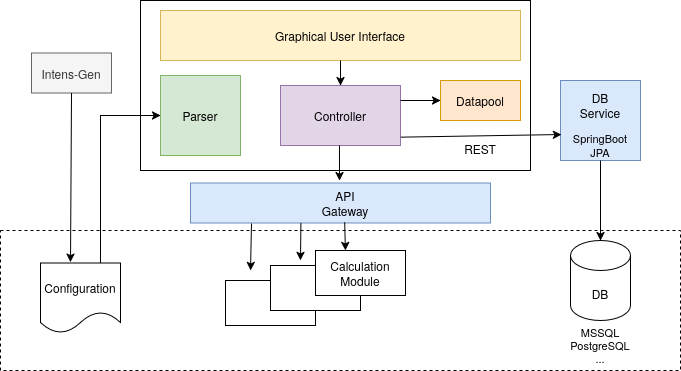
\includegraphics[width=0.52\linewidth]{intens-arch.drawio}
\hfill
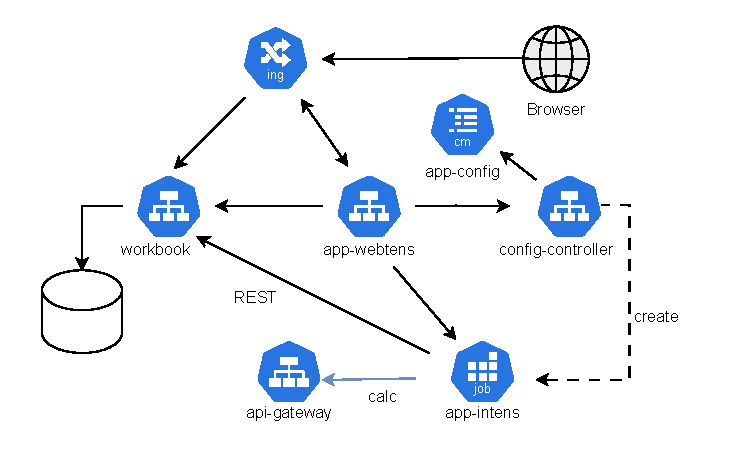
\includegraphics[width=0.47\linewidth]{k8s-intens.drawio}
  \caption{Architecture in Desktop and Cloud Operation Mode}
\end{figure}
\index{overview} \index{architecture}
\vspace {0.1cm}

Each INTENS application is created through a simple script which contains
the configuration of the applications data and the interfaces
of DB Service, calculation programs and user interface. The operation
of INTENS applications is possible in a desktop or in a cloud enviroment.
%as docker containers.

As shown in the above figure, INTENS consists of the following components:
\begin{description}
\index{Parser!architecture}
\item[The Parser] interpretes the configuration data at program startup
  and sends the appropriate messages to all involved objects to create
  the application with all configured interfaces.
%%
\index{DATAPOOL@\DATAPOOL!architecture}
\item[The Datapool] dynamically manages an arbitrary number of variables
   with an arbitrary number of calculation variants, called cycles.
   The only limitation is the size of the machine's virtual memory.
   The variables have unique names, data types (INTEGER, REAL or STRING)
   and modification attributes (OPTIONAL, EDITABLE, LOCKABLE) but
   no static dimension. They can be accessed as lists (vectors) or matrices
   with dynamic dimension, which will be expanded or reduced according to
   the requested size.
%%
\index{UI\_MANAGER@\UIMANAGER!architecture}
\item[The UI Manager] creates the necessary dialog objects, manages
  the user input and displays the results to provide a standardized
  and uniform look-and-feel. Each application has
  one main window, a configurable number of form windows and several
  dialog windows like file selection dialogs and message dialogs.
  The main window contains
  a title bar, a menu bar, a work area and an action button bar.
  The values of the data items
  are displayed in textfields which are part of the form windows. Each form
  consists of an configurable number of fieldgroups, text and plot windows,
  which can be arranged horizontally and vertically within one form.
  Plot graphs can be printed and/or saved as PostScript or HPGL files.
  Calculation programs can be started and stopped by activating
  push buttons or menu buttons.
%%
\index{STREAMER@\STREAMER!architecture}
\item[The Streamer] manages all input and output formats. A stream consists
  of a sequence of data items and string constants. Together with the
  datapool and the operator, the streamer also controls the dependencies
  between the datapool items. In order to keep the data consistent,
  all data items that belong to an output stream are set invalid
   if one of the items of a corresponding input stream is modified.
%%
\index{OPERATOR@\OPERATOR!architecture}
\item[The Operator] communicates with the operating system and the
  external calculation programs using the pipe mechanism or the
  MathLink protocol. Several (one to many) calculation programs
  are combined to a process group that can be started and stopped
  by the user activating a push button. Data can also be read from
  and saved to files.
%%
\end{description}
